\chapter{Closed-Loop Subspace Identification of a Quadrotor}\label{results}
\section{Identification Results}
Using closed-loop input-output data captured from test flights of a quadrotor operating under PRBS inputs, we developed an LTI system model using subspace identification techniques with innovation estimation following the procedure outlined in Chapter \ref{approach}.

\subsection{Experimental Data Used for Identification}
We conducted many test flights and ultimately identified 18 data sequences of high enough quality to use for model identification and verification. Of these sequences, nine were collected with the vehicle operating under PRBS inputs and nine were collected with the vehicle operating under individual degree of freedom  excitation inputs (three each for pitch, roll, and yaw). While we considered concatenating multiple data sequences together into a longer single input-output sequence, models identified with an individual sequence proved to adequately capture desired system dynamics.


\subsection{Model Order Selection}
System order selection occurs as a part of the model identification procedure. A plot of the singular values of the extended observability matrix, shown in Figure \ref{singular_values} is intended to provide a visual means to select the best system order. 
\begin{figure}[hbt!]
	\centering
	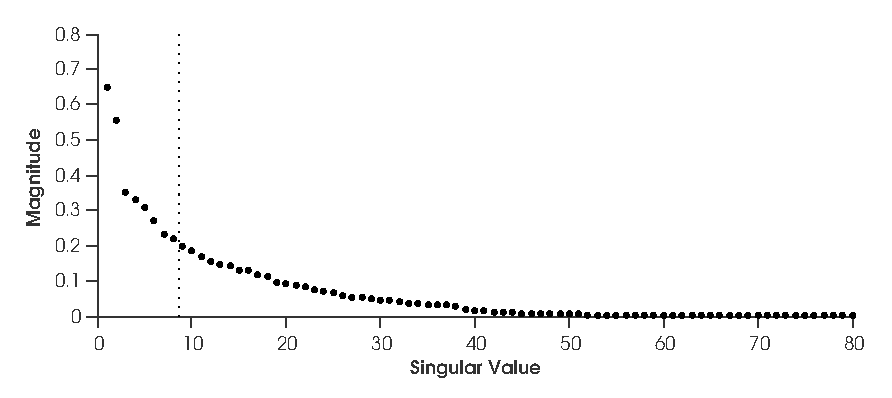
\includegraphics{../fig/singular_values_parsim.eps}
	\caption{A plot of the singular values of the extended observability matrix, used to determine the model order. The vertical dotted line shows the partitioning location between system response and noise in the final eighth order model.}
	\label{singular_values}
\end{figure}

From the figure, we see a significant drop in the magnitude of the singular values after the second singular value, but selecting a system order of two did not adequately model the system dynamics. As a result, we tested a number of models with orders ranging from 3 to 12 and ultimately selected an 8th order model for its consistent modeling of system dynamics from multiple PRBS data sets.

\subsection{Past and Future Horizon for Innovation Estimation}
Estimation of the innovation sequence requires the definition of past and future estimation horizons. Following the procedure outlined in Section \ref{sec:past_and_future_horizon_selection}, we settled on a past estimation horizon of 60 and a future estimation horizon of 17. 

By plotting the poles of all evaluated models (Figure \ref{fig:poles_all}), we see the most common pole locations. The poles of the final system model, plotted in Figure \ref{fig:poles_1760} show the model is stable and only one pole has an oscillatory response (the pole is located in the left half of the real plane). This is in contrast to the full set of models, which most commonly have three poles exhibiting an oscillatory response. The single oscillatory pole in the final system model is also faster than each of the three poles common to the set of all models, increasing the overall responsiveness of the final model. 

\begin{figure}[htb!]
	\centering
	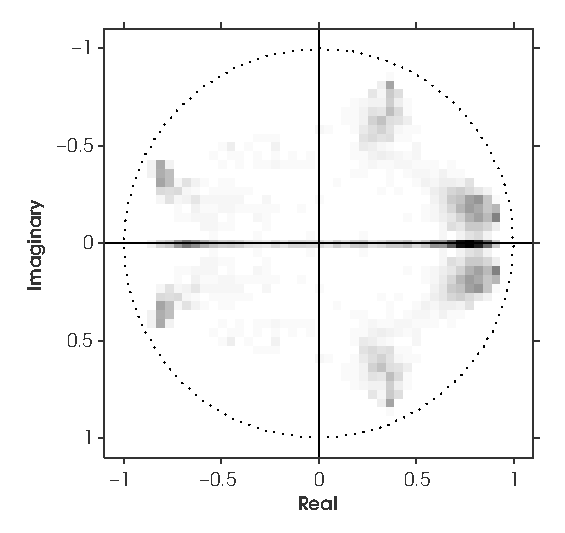
\includegraphics{../fig/poles_all.eps}
	\caption{Pole distribution of 8th order models generated for 756 combinations of past and future horizons. Darker shading indicates higher pole concentrations.}
	\label{fig:poles_all}
\end{figure}

\begin{figure}[htb!]
	\centering
	\includegraphics{../fig/poles_1760.eps}
	\caption{Poles of final 8th order model.}
	\label{fig:poles_1760}
\end{figure}


\subsection{Identified 6DOF Quadcopter Model}
The final 8th order quadrotor LTI model identified using innovation estimation, given in its state space form is 
\begin{subequations}\label{eq:2_lti}
\begin{equation*}x(k+1) = Ax(k) + Bu(k)\end{equation*}
\begin{equation*}y(k) = Cx(k) + Du(k)\end{equation*}
\end{subequations}
where system input $u = \begin{bmatrix}u_1 & u_2 & u_3 & u_4\end{bmatrix}^T$ is a vector of motor commands and system output $y = \begin{bmatrix}\ddot x & \ddot y & \ddot z & p & q & r\end{bmatrix}^T$ is a vector of accelerometer and gyroscope measurements. The system matrices of the model appear fully in Table \ref{identified_system_matrices}.

\begin{table}[!htb]
\centering
\caption{Identified System Matrices, 8th order LTI Quadrotor Model}%\vspace{0.5em}
\fbox{
\begin{minipage}{5.5in}
\footnotesize % DECREASE FONT SIZE
\begin{equation*}
A = \begin{bmatrix}
0.8521&-0.0304&-0.2107&0.3639&0.0859&-0.2501&0.0172&-0.0448\\
-0.0794&0.7874&0.1238&0.2699&0.4075&0.0408&-0.3177&-0.0088\\
0.1025&-0.0053&0.5120&-0.4573&0.3561&-0.5139&0.0986&-0.1669\\
-0.0379&0.0325&-0.5483&-0.3013&0.4049&-0.0075&0.1634&0.3805\\
0.0042&-0.0926&0.0224&0.1017&0.5170&0.3392&0.5775&-0.2288\\
0.1567&-0.0832&0.5616&0.2255&-0.0186&0.3945&0.2078&0.4095\\
0.0077&0.0579&0.0469&0.0398&-0.0686&-0.2426&-0.0026&0.2523\\
-0.0622&0.0535&-0.0811&0.0428&0.1020&-0.0254&0.0795&0.4353
\end{bmatrix}
\end{equation*}
\begin{equation*}
B = \begin{bmatrix}
-0.0025&-0.0037&-0.0112&-0.0017\\
0.0022&0.0027&0.0039&0.0045\\
-0.0038&-0.0018&0.0101&-0.0024\\
0.0098&0.0090&-0.0020&0.0037\\
-0.0011&0.0063&-0.0035&0.0027\\
0.0077&0.0107&0.0038&0.0054\\
-0.0009&-0.0085&-0.0032&-0.0058\\
-0.0013&-0.0042&-0.0072&-0.0047
\end{bmatrix}
\end{equation*}   
\begin{equation*}
C = \begin{bmatrix}
-0.0001&0&-0.0001&0.0001&-0.0001&0.0002&0.0003&-0.0003\\
0&0&0.0001&-0.0001&0.0002&-0.0001&-0.0002&0.0003\\
0.0001&-0.0001&0&0&-0.0002&0.0003&0.0000&-0.0004\\
-0.0252&-0.5396&0.0367&0.0661&0.4731&0.1647&-0.6491&0.0088\\
-0.4569&-0.2298&-0.0069&0.6147&0.1088&-0.5000&0.1831&0.0206\\
-0.0116&0.0591&0.0035&0.0091&0.0085&-0.0450&0.0297&-0.0022
\end{bmatrix}
\end{equation*} 
\begin{equation*}
D = \begin{bmatrix}
0&0&0&0\\
0&0&0&0\\
0&0&0&0\\
0&0&0&0\\
0&0&0&0\\
0&0&0&0
\end{bmatrix}
\end{equation*}
\normalsize % INCREASE FONT SIZE
\end{minipage}}
\label{identified_system_matrices}
\end{table}



%Stimulating the system with a step response provides insight into the model performance (Figure \ref{fig:5_step}).
%\begin{figure}[htb!]\label{fig:5_step}
%	\centering
%	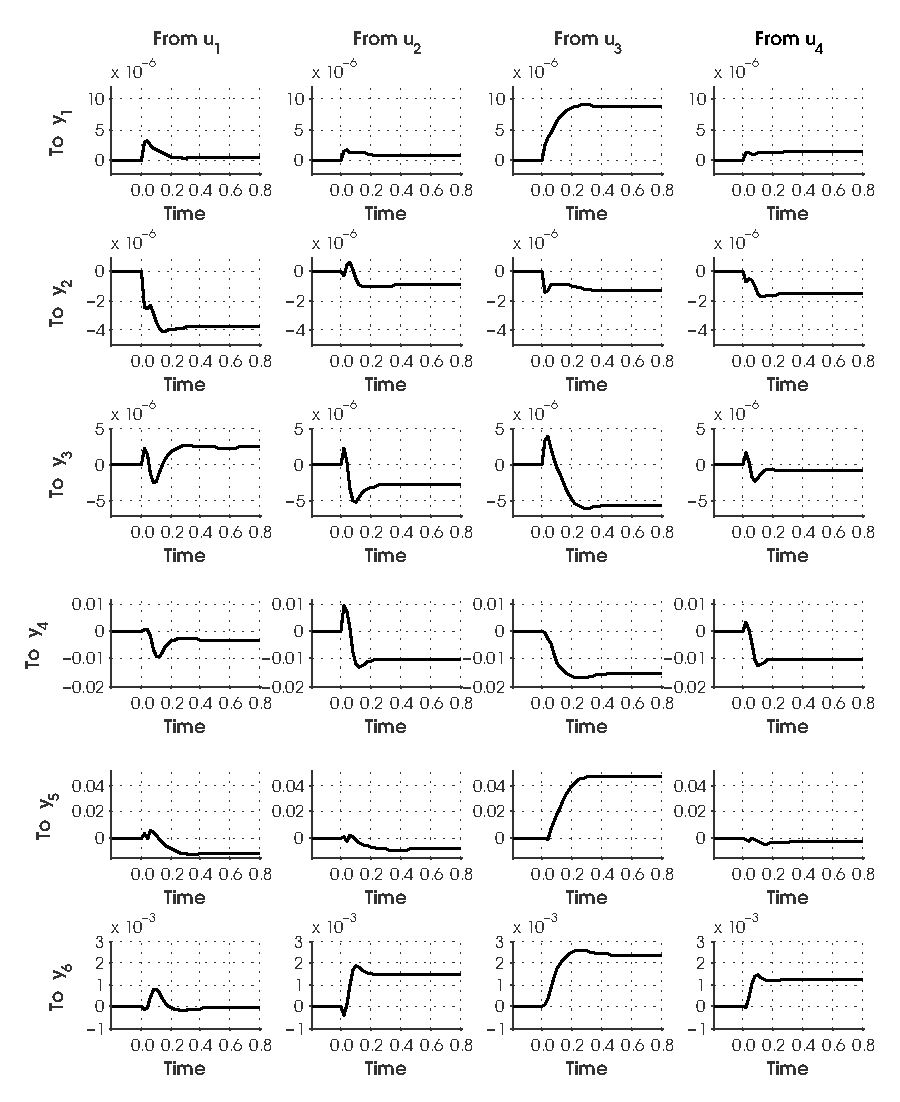
\includegraphics{../fig/step_resp_parsim.eps}
%	\caption{Step response of the 8th order system model.}
%\end{figure}\clearpage






\newpage
\section{Time Domain Model Validation}
Comparing system response predicted by the identified model with measured system response originating from the same input sequence provides a straightforward way to validate the identified model in the time domain. We compared the identified model's time domain response with the measured response of the physical system using four different input sequences: PRBS input, pure pitch input, pure roll input, and pure yaw input. 

Because the IEM deals with the coupling between system input and past noise present in a closed-loop system by pre-estimating the noise sequence from the input-output data used for identification, some true system dynamics are inevitably ``estimated out'' of the model during this procedure. This is evident in the fact that some of the faster system modes are not perfectly represented by the model.

By also evaluating the identified model's ability to represent the decoupled dynamics of the physical system, we are able to draw conclusions about the ability of a PRBS input sequence to identify individual dynamical modes of a system. 

\subsection{Evaluation of Full 6DOF LTI Model Dynamics}
Figure \ref{sim_1760_20131017212626_31_38500} shows the comparison of system response between the identified model and the physical system. In general, the identified model provides a satisfactory estimate of the physical system dynamics. The pitch and roll rates are accurately predicted and the magnitudes of the $x$, $y$, and $z$ accelerations are correctly predicted. 

While the system acceleration predictions are accurate with respect to the magnitude of acceleration, it is not surprising that the predictions do not more closely follow the measured response. This is due to the fact that the accelerometers are very susceptible to measuring vehicle vibrations caused by slightly unbalanced motors and propellers. Because these vibrations occur at a much higher frequency than the Nyquist frequency, they are not captured by the identified model and thus not reflected in the system response.

Inspecting the yaw rate response, we see that the model does not accurately capture the yaw dynamics of the physical system. We observed this deficiency in all verification tests when comparing simulated model response with the measured response of the physical system. We hypothesize that this failure to successfully identify the yaw dynamics is in part due to the way a quadrotor's yaw mode is excited. While the pitch and roll modes of a quadrotor are excited by changing the rotor speed of only two opposing rotors, excitation of the yaw mode requires speed changes to all four rotors. It is possible that a higher order system model would capture these dynamics, although we tested models up to 12th order without success. This problem is not isolated; others (\cite{lee2011attitude} and \cite{mettler2000system}) have experienced similar difficulties identifying yaw dynamics in rotorcraft through system identification.

\subsection{Evaluation of LTI Model Pitch Dynamics}
Figure \ref{sim_1760_pitch} shows the comparison of system response between the identified model and the physical system excited by pure pitch inputs. The simulated pitch rate aligns with the measured value showing that the model accurately represents isolated pitch dynamics of the system.


\subsection{Evaluation of LTI Model Roll Dynamics}
Figure \ref{sim_1760_roll} shows the comparison of system response between the identified model and the physical system excited by pure roll inputs. The simulated roll rate generally tracks with the measured value. In several places, the measured roll rate is clipped while the predicted value is not clipped (in particular between 1.5 and 2 seconds). This is likely due to nonlinearities in the physical system not captured by the linear model.


\subsection{Evaluation of LTI Model Yaw Dynamics}
Figure \ref{sim_1760_yaw} shows the comparison of system response between the identified model and the physical system excited by pure yaw inputs. The identified model does not accurately capture the isolated yaw dynamics of the physical system. This is expected, as the model also failed to adequately represent the yaw dynamics of the full 6DOF system operating under PRBS input. Inspection of the pitch and roll rate responses in Figure \ref{sim_1760_yaw} reveals a coupling between yaw input and simulated pitch and roll rate. Both yaw inputs beginning at 1.7 seconds and 2.2 seconds result in responses in simulated pitch and roll rates, an effect is not seen in the physical system. The yaw dynamics are not completely missed however. From Figure \label{sim_1760_20131017212626_31_38500} we see that after 2 seconds, the simulated response somewhat tracks with the measured output for small angle changes.







\newpage
\begin{figure}[htb!]
	\centering
	\includegraphics{../fig/sim_1760_20131017212626_31_38500.eps}
	\caption{Simulated response (dashed) of identified 8th order LTI system model compared with measured system response (solid). Both systems were stimulated with an identical PRBS input sequence.}
	\label{sim_1760_20131017212626_31_38500}
\end{figure}\clearpage

\newpage
\begin{figure}[htb!]
	\centering
	\includegraphics{../fig/sim_1760_pitch.eps}
	\caption{Simulated (dashed) response of identified model to pitch input compared with measured system response (solid).}
	\label{sim_1760_pitch}
\end{figure}\clearpage

\newpage
\begin{figure}[htb!]
	\centering
	\includegraphics{../fig/sim_1760_roll.eps}
	\caption{Simulated (dashed) response of identified model to roll input compared with measured system response (solid).}
	\label{sim_1760_roll}
\end{figure}\clearpage

\newpage
\begin{figure}[htb!]
	\centering
	\includegraphics{../fig/sim_1760_yaw.eps}
	\caption{Simulated (dashed) response of identified model to yaw input compared with measured system response (solid).}
	\label{sim_1760_yaw}
\end{figure}\clearpage


\newpage
\section{Comparing Identified Model Performance From PO-MOESP and IEM Algorithms With Closed-Loop Data}
In addition to evaluating the performance of a model identified using a closed loop subspace identification method (IEM), we analyzed the performance of a model identified from the same closed-loop data using a traditional subspace identification method which makes no attempt to correct for the presence of closed-loop data (PO-MOESP). Because we used the same input-output data to develop both models, the only differences between the two models are due to the identification algorithms used. 

Unlike IEM, the PO-MOESP algorithm assumes no correlation between system input an past noise (an invalid assumption in this case), with the effect of violating this assumption easily seen in Figure \ref{sim_1760_moesp.eps}. Because PO-MOESP makes no attempt to deal with the coupling between the input and noise terms however, the model identified using PO-MOESP does not suffer from the issue of having true system dynamics pre-estimated out. The result is that although the magnitudes of estimated system responses are incorrect, the model identified using PO-MOESP tracks the true system better than the IEM model in some cases. Despite this fact, the IEM model provides a more correct representation of the overall dynamics of the physical system in the presence of closed-loop data.

\newpage
\begin{figure}[htb!]
	\centering
	\includegraphics{../fig/sim_1760_moesp.eps}
	\caption{Simulated (dashed) response of identified model to yaw input compared with measured system response (solid). IEM results are plotted in light gray (solid) for reference.}
	\label{sim_1760_moesp.eps}
\end{figure}\clearpage











